\section{建模方法}
\label{sec:prelims}

我们扩展了 \textcite{ingrosso2022data} 的设定,
这是一个神经网络的最小示例,能够从理想化的自然数据中学习局部感受野。
我们在 \cref{sec:theory} 中分析了这个设定中学习的动态,
并在 \cref{sec:experiments} 中通过仿真验证了我们的分析模型。
\subsection{神经网络架构与学习算法}
\label{sec:model}

我们考虑一种具有非线性激活函数和标量输出的两层前馈神经网络。尽管结构简单,该架构却具有很强的表达能力,能够在适当缩放下逼近任意可积的一元函数~\parencite{barron1993universal, pinkus1999approximation},并展现出丰富的特征学习动态,这些动态是大规模模型性能的基础~\parencite{woodworth2020kernel},使得该架构持续成为神经网络理论分析的研究对象~\parencite{mei2018mean, goldt2019dynamics, veiga2022phase}。我们将一个输入维度为 $N$、隐藏单元数为 $M$、输出为一维标量的两层网络表示为
\newcounter{modelenumi}
\begin{model}{\textbf{模型 1} (\emph{多神经元架构})}{}
\begin{enumerate}[series=modelenumi]
  \item \label{item:many-neuron-model}
    \makebox[\linewidth - 2.5em]{
      $\hat{y}(\mathbf{x}) = b^{(2)} + \sum_{m=1}^M w_m^{(2)}
      \sigma\left(b_m^{(1)} + \langle \mathbf{w}_m^{(1)}, \mathbf{x} \rangle \right)$
    }
\end{enumerate}
\end{model}
其中,$\sigma : \R \to \R$ 是逐点非线性函数,如修正线性单元(ReLU)或 sigmoid 函数,
$\mathbf{w}_m^{(1)} \in \R^N$ 和 $w_m^{(2)} \in \R$ 是可学习的权重,
$b_m^{(1)}, b^{(2)} \in \R$ 是可学习的偏置项,$\langle \cdot, \cdot \rangle$ 表示 $\R^N$ 上的标准欧几里得内积(点积)。
当第二层参数固定时,该模型被称为 \emph{软委员会机}~\parencite[SCM;][]{saad1995line},
正如~\parencite{ingrosso2022data} 所指出的那样,该模型学习到的感受野噪声更小,但呈现出类似的局部化行为。
在我们\textbf{仿真实验}~(\cref{sec:experiments})中,关注的是 \labelcref{item:many-neuron-model} 中的多神经元架构,
但即使在本文考虑的理想自然数据模型下,该模型的动态也过于复杂,难以直接分析。
为了推导\textbf{解析}结果~(\cref{sec:theory}),我们考虑能够展现所需局部化现象的最简单神经网络:一个没有偏置项、采用 ReLU 激活函数的单隐藏神经元模型,表示为
\begin{model}{\textbf{Model 2} (\emph{single-neuron architecture}).}{}
\begin{enumerate}[resume*=modelenumi]
  \item \label{item:single-neuron-model}
    \makebox[\linewidth - 2.5em]{
      $\hat{y}(\mathbf{x}) =
      \operatorname{ReLU}\left(\langle \mathbf{w}, \mathbf{x} \rangle \right)$
    }
\end{enumerate}
\end{model}
其中 $\operatorname{ReLU}(x) = \max(x,0)$,逐点作用于向量输入。
如 \textcite{ingrosso2022data} 所示,由 \labelcref{item:many-neuron-model,item:single-neuron-model} 所定义的多神经元与单神经元模型学习到的局部化感受野在空间平移下具有相似的定性特征,
这使我们能够将对单神经元~\labelcref{item:single-neuron-model} 学习动态的分析推广至多神经元模型~\labelcref{item:many-neuron-model}。
在仿真中,我们将权重与偏置初始化为来自具有缩放方差的各向同性高斯分布的独立样本,
并使用固定学习率的批量梯度下降算法,在任务输入输出对上最小化均方误差(MSE);任务采样过程见 \cref{sec:task}。
\subsection{刺激特性}
\label{sec:input}

\textcite{ingrosso2022data} 的数据模型
可以证明满足三个条件,这些条件使我们能够在 \cref{sec:theory} 中进行分析。
我们考虑了几个其他的数据模型,这些模型具有以下特性,但在生成机制上有所不同,
目的是探讨这些特性对定位的影响。
特别地,我们考虑从 $\R^N$ 上分布 $p$ 中采样的数据 $\mathbf{X}$,满足以下条件:
\newcounter{propenumi}
\begin{stimulus}{\textbf{刺激属性 1--3} (\emph{自然图像的理想化})}{}
\begin{enumerate}[series=propenumi]
  \item \label{item:weak-dependence} (位置) 弱依赖性:对于任何固定的 $\rho \in (0,1)$,当 $N \to \infty$ 时,
    $$\alpha(N) \triangleq \sup_{A \subseteq \R, B \subseteq \R^{(1-\rho) N}} |\PR(X_1 \in A, X_{> \rho N} \in B) - \PR(X_1 \in A) \PR(X_{> \rho N} \in B)| \to 0~,$$
  \item \label{item:translation-invariance} 平移不变性:对于所有 $\mathbf{x} \in \R^N$,有 $p(\mathbf{X} = \mathbf{x}) = p(\mathbf{X} = \mathcal{S} \mathbf{x})$,其中 $\mathcal{S}$ 是圆形移位算子,
  \item \label{item:sign-symmetry} 符号对称性:对于所有 $\mathbf{x} \in \R^N$,有 $p(\mathbf{X} = \mathbf{x}) = p(\mathbf{X} = -\mathbf{x})$。
\end{enumerate}
\end{stimulus}
属性~\labelcref{item:weak-dependence,item:translation-invariance}
是自然图像数据的定义特征~\parencite{hyvarinen2009natural}。
属性~\labelcref{item:sign-symmetry}
也可以通过去中心化自然图像后得到,并且在分析上是方便的,
因为它意味着 $\E[\mathbf{X}] = 0$。
属性~\labelcref{item:weak-dependence} 假设 $p$ 由 $N$ 隐式参数化,
以便说明 $\mathbf{X}$ 的条目之间的统计依赖随着它们的分离增大而消失。\smash{\footnotemark}\footnotetext{
  \labelcref{item:weak-dependence} 中的弱依赖条件基于强 $\alpha$-混合性,这是 \cite{rosenblatt1956central} 首次提出的一个概念,
  用于获得中心极限定理的推广,之后我们会用到。
  我们选择 $\alpha$-混合性,因为它容易解释和验证,
  但也可以使用弱依赖的其他定义 \parencite[\eg][]{bardet2008dependent}。
}

我们将 $\mathbf{X}$ 的协方差记为 $\Sigma \triangleq \operatorname{Cov}[\mathbf{X}]$,
主对角线条目的平方(即每个条目的方差)记为 $\sigma^2$,
第 $i$ 行记为 $\sigma_i$。
弱依赖(\labelcref{item:weak-dependence})意味着 $\Sigma$ 的主对角线远离的条目将为 0,
而平移不变性(\labelcref{item:translation-invariance})意味着 $\Sigma$ 是循环矩阵(即沿每条对角线的条目相等),
因此可以通过单行来识别;见 \cref{fig:task}(中)。
\subsection{长度尺度判别任务}
\label{sec:task}

\textcite{ingrosso2022data} 开发了一个最小化任务,在该任务中,定位在前馈神经网络中出现:在两个分布之间进行二元判别,这些分布的输入在其条目之间的相关性的长度尺度上有所不同。
这个长度尺度判别任务可以看作是自监督学习~\parencite{kolesnikov2019revisiting,chen2020simple} 表示的前置任务~\parencite[\cf~无监督:][]{olshausen1996emergence,bell1997independent}。
更精确地说,我们根据以下方式生成数据 $(\mathbf{X},Y)$ 用于监督训练:
\begin{align} \label{eq:task}
    \mathbf{X} \mid Y = y \sim p(\mathbf{X};\Sigma_y)~,
\end{align}
其中 $p$ 待定义,$\Sigma_y$ 是每个 $y$ 对应的不同协方差矩阵,我们从一组递增的 \emph{长度尺度相关类} $y \in \{0,1,\ldots\}$ 中均匀抽样,表示远距离位置之间相关性的强度。
例如,在两个类别的情况下($y = 0, 1$),我们令 $\Sigma_0$ 比 $\Sigma_1$ 更接近 $\sigma^2 \mathbb{I}_N$,其中 $\mathbb{I}_N$ 是 $N \times N$ 的单位矩阵,$\sigma$ 是一个固定值。
这种构造通过为每个类别提供不同的协方差矩阵,隔离了二阶统计量,正如我们将在下文中看到的那样,这些统计量与 $p(\mathbf{X})$ 的其他属性分别进入学习动态,最关键的是其隐含的边际分布 $p(X_i)$。

\paragraph{\texttt{Ising}.}\hspace{-2pt}
我们考虑的第一个分布是一维伊辛模型。
它作为一种分布具有兴趣,因为它满足 \labelcref{item:weak-dependence,item:translation-invariance,item:sign-symmetry},其边际分布 $p(X_i)$ 在 $\{ \pm 1 \}$ 上有极端支持,
使其成为最强烈促进定位的分布,正如我们将在 \cref{sec:theory} 中看到的那样。
在没有外部场的情况下,伊辛分布为
\begin{equation}
    p_\text{\texttt{Ising}}(\mathbf{X}=\mathbf{x})
    = p_\text{\texttt{Ising}}(X_1=x_1,\ldots,X_N=x_N) = e^{ -\sum_{i=1}^{N} J x_i x_{i+1} } / \mathcal{Z},
\end{equation}
其中 $J$ 是选择的二元相互作用强度,$\mathcal{Z}$ 是归一化常数,我们通过 $x_{N+1} \equiv x_1$ 强制周期边界约束。
随着 $J$ 的增加,$\mathbf{X}$ 中的相关性长度尺度也增加。
在仿真中,我们使用 Gibbs 采样器~\parencite{geman1984stochastic} 从 $p_\texttt{Ising}$ 中抽样。
仿真中的判别任务在
\cref{sec:experiments}
中使用 $J_1=0.7$(对于 $y=1$)和 $J_0=0.3$(对于 $y=0$)。

\newcommand{\sampleheight}{42pt}
\newcommand{\covheight}{46pt}
\newcommand{\marginalheight}{50pt}
\setlength{\tabcolsep}{4pt}
\begin{figure}[t]
  \centering
  \hspace{-1.2em}
  \scalebox{0.9}{
  \begin{centering}
    \begin{tabular}{p{51pt}
      @{\hspace{10pt}}m{2pt}l
      @{\hspace{5pt}}l
      @{\hspace{10pt}}m{2pt}l
      @{\hspace{10pt}}m{2pt}l}
        \raisebox{18pt}{\small$\texttt{Ising}$} &
        \raisebox{34pt}{\rotatebox{90}{\tiny input value}} &
        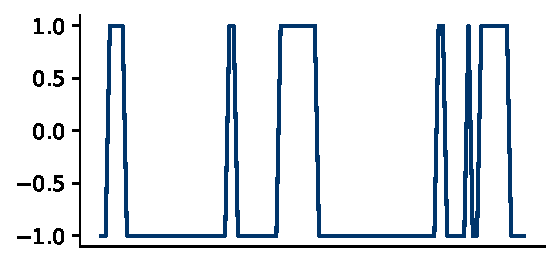
\includegraphics[height=\sampleheight]{figures/task/samples_long/ising.pdf} &
        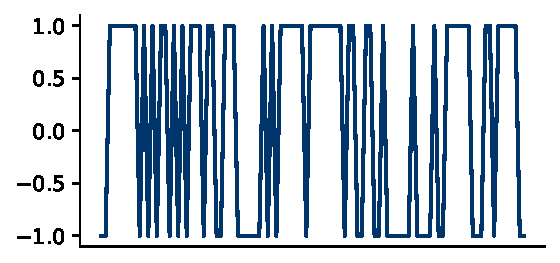
\includegraphics[height=\sampleheight]{figures/task/samples_short/ising.pdf} &
        \raisebox{38pt}{\rotatebox{90}{\tiny input dimension}} &
        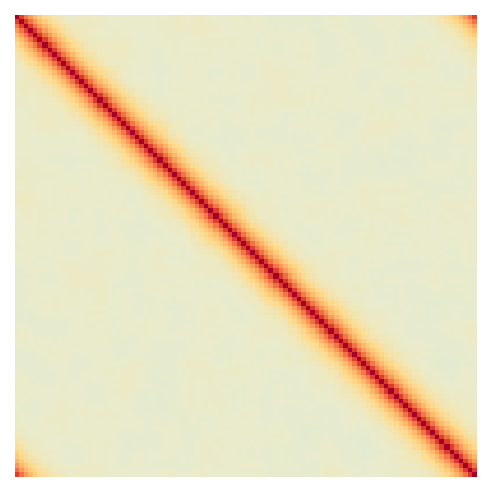
\includegraphics[height=\covheight]{figures/task/cov/ising.pdf} &
        \raisebox{40pt}{\rotatebox{90}{\tiny $p(X_i)$}} &
        \raisebox{-4pt}{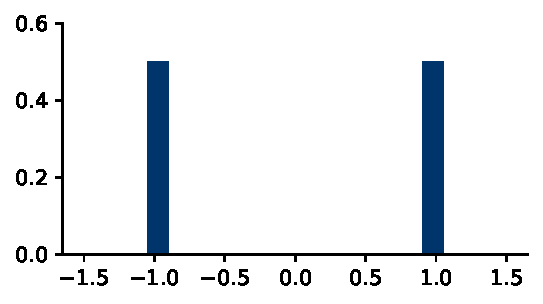
\includegraphics[height=\marginalheight]{figures/task/marginal/ising.pdf}} \\
        \noalign{\vskip -36pt}
        \raisebox{18pt}{\small$\texttt{NLGP}(0.01)$} &
        \raisebox{34pt}{\rotatebox{90}{\tiny input value}} &
        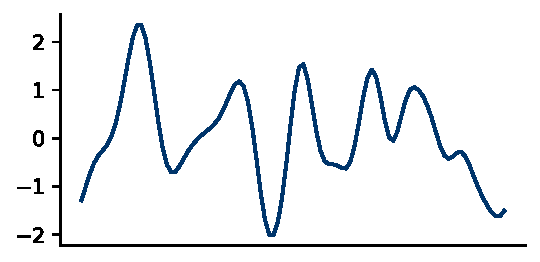
\includegraphics[height=\sampleheight]{figures/task/samples_long/gaussian.pdf} &
        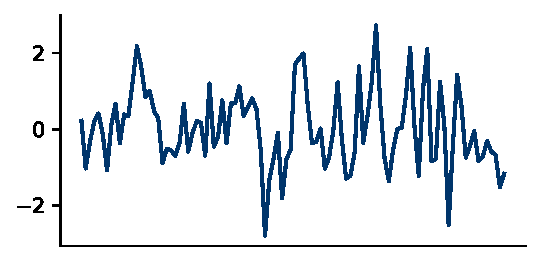
\includegraphics[height=\sampleheight]{figures/task/samples_short/gaussian.pdf} &
        \raisebox{38pt}{\rotatebox{90}{\tiny input dimension}} &
        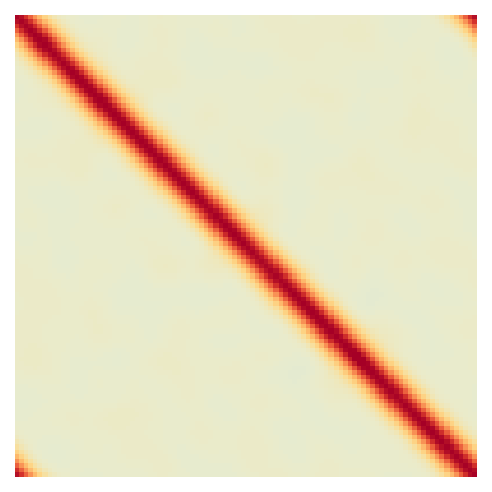
\includegraphics[height=\covheight]{figures/task/cov/gaussian.pdf} &
        \raisebox{40pt}{\rotatebox{90}{\tiny $p(X_i)$}} &
        \raisebox{-4pt}{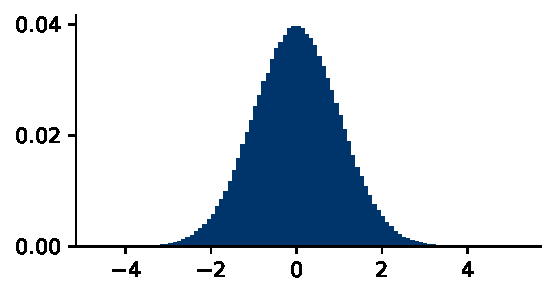
\includegraphics[height=\marginalheight]{figures/task/marginal/gaussian.pdf}} \\
        \noalign{\vskip -36pt}
        \raisebox{18pt}{\small $\texttt{Kur}(5)$} &
        \raisebox{34pt}{\rotatebox{90}{\tiny input value}} &
        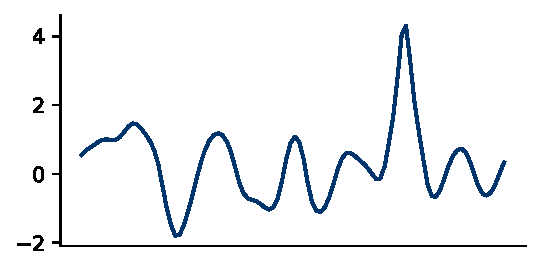
\includegraphics[height=\sampleheight]{figures/task/samples_long/alg5.pdf} &
        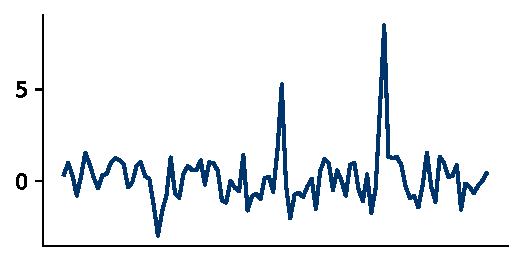
\includegraphics[height=\sampleheight]{figures/task/samples_short/alg5.pdf} &
        \raisebox{38pt}{\rotatebox{90}{\tiny input dimension}} &
        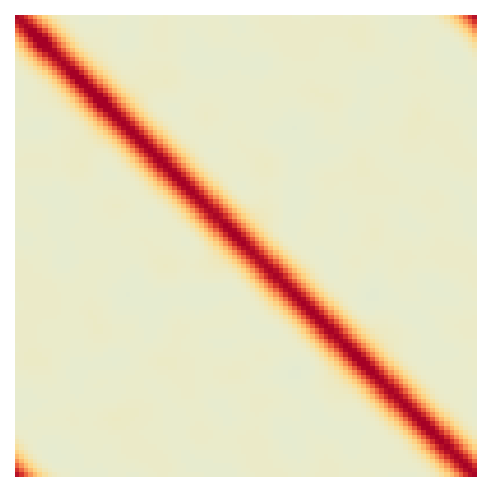
\includegraphics[height=\covheight]{figures/task/cov/alg5.pdf} &
        \raisebox{40pt}{\rotatebox{90}{\tiny $p(X_i)$}} &
        \raisebox{-4pt}{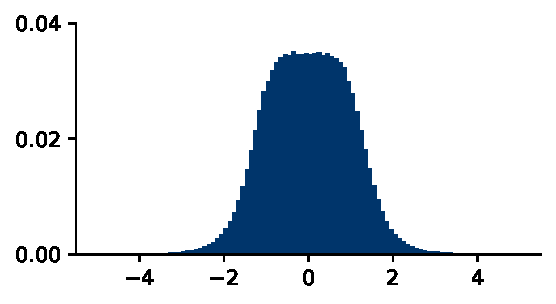
\includegraphics[height=\marginalheight]{figures/task/marginal/alg5.pdf}} \\
        \noalign{\vskip -37pt}
        &&
        \hspace{25pt}\tiny input dimension &
        \hspace{25pt}\tiny input dimension & &
        \hspace{3pt}\tiny input dimension & &
        \hspace{37pt}\tiny input value \\
  \end{tabular}
  \end{centering}
  }
  \caption{
    从左到右:
    长尺度和短尺度样本 $\mathbf{x}$,
    单一尺度的协方差 $\Sigma$,
    以及数据模型的边缘分布 $p(X_i)$,如 \cref{sec:task} 所述:
    Ising 模型(左、右样本分别为 $J=1.2, 0.3$),
    非线性高斯过程~\parencite[NLGP;~][]{ingrosso2022data},
    以及可控峰度模型 \texttt{Kur}
    (左、右样本分别为 $\xi=5, 1$)。
    \emph{
    每个模型生成的样本以零为中心,且其协方差可以被约束为相似,
    但具有不同的高阶统计量,从维度方向的边缘分布中可以看出这一点。
    }
}
  \label{fig:task}
  \vspace{-10pt}
\end{figure}


\paragraph{\texttt{NLGP}$(g)$.}\hspace{-2pt}
我们还考虑了 \textcite{ingrosso2022data} 中使用的数据模型——非线性高斯过程(NLGP),它通过一个单一参数 $g$ 使我们能够在会和不会导致定位的分布之间进行插值。
从 NLGP 中,给定 $Y = y$,采样一个样本 $\mathbf{X}$ 的构造方式是,首先从高斯分布采样 $\mathbf{Z} \mid Y = y \sim \NN(0, \tilde{\Sigma}_y)$,然后通过以下方式进行变换:
\begin{equation} \label{eq:nlgp}
    X_i \triangleq \operatorname{erf}(g Z_i) / \mathcal{Z}(g) \qquad 1 \leq i \leq N,
\end{equation}
其中 $\operatorname{erf}$ 是高斯误差函数,$\mathcal{Z}$ 是归一化常数,确保 $X_i$ 和 $Z_i$ 的方差相同,$\tilde{\Sigma}_y$ 是 $\mathbf{Z}$ 的协方差矩阵,我们使用 $(\tilde{\Sigma}_y)_{ij} = \exp(-(i-j)^2/\xi^2)$ 作为长度尺度参数 $\xi$ \cite{ingrosso2022data}。
如果 $g \approx 0$(即没有观察到定位),$g Z_i$ 将趋向于 $\operatorname{erf}$ 的线性区域,因此 $Z_i$ 将不被变换,即 $\mathbf{X}$ 是高斯分布。
然而,当 $g \to \infty$(即观察到定位时),$g Z_i$ 将趋向于饱和 $\operatorname{erf}$,因此 $X_i$ 将支持 $\{ \pm 1 \}$。

\paragraph{\texttt{Kur}$(k)$.}\hspace{-2pt}
我们考虑的最后一个模型家庭使我们能够灵活控制边际分布 $p(X_i)$ 的峰度 $\kappa$。
在伊辛模型中,边际分布的 \emph{超额}峰度($\kappa - 3$)固定为 $-2$,而在 $\texttt{NLGP}(g)$ 中,它从 $-2$ 变化到 $0$。
这个模型家庭允许我们将超额峰度从负值变化到正值。
我们通过逆变换采样从这个家庭中抽样 $\mathbf{X} \mid Y = y$,以在强制依赖关系的同时改变边际分布,使用高斯 Copula。
更具体地说,我们首先从高斯分布中抽样 $\mathbf{Z} \mid Y = y \sim \NN(0, \tilde{\Sigma}_y)$,然后通过以下方式进行变换:
\begin{equation}
    X_i \triangleq f^{-1}( \Phi( Z_i / \tilde{\sigma} )) / \mathcal{Z}, \qquad 1 \leq i \leq N, \label{eq:alg}
\end{equation}
其中 $\tilde{\sigma}$ 是 $Z_i$ 的标准差,$\Phi$ 是标准高斯累计分布函数(CDF),$f$ 是 $X_i$ 的期望边际分布的 CDF,$\mathcal{Z}$ 是归一化常数,我们通过数值方法计算该常数。
我们将 $\tilde{\Sigma}_y$ 定义为与 $\texttt{NLGP}$ 相同。
我们选择 $f$ 为广义的 \emph{代数 Sigmoid} 函数(见 \cref{sec:algebraic-sigmoid}),对于 $k > 0$,利用其可解的反函数,简化了 \cref{eq:alg} 中的过程。
我们将相应的分布表示为 $\texttt{Kur}(k)$。
尽管我们能够连续变化超额峰度,但我们没有显式的形式;然而,数值计算表明,对于 $k \lessapprox 5.8$,超额峰度为正,而对于 $k \gtrapprox 5.9$,它为负。
